\chapter{Training einer KI}
\label{chap:training}

In diesem Kapitel werden wir lernen, wieso und wie eine KI funktioniert.

\begin{figure}[h]
    \centering
    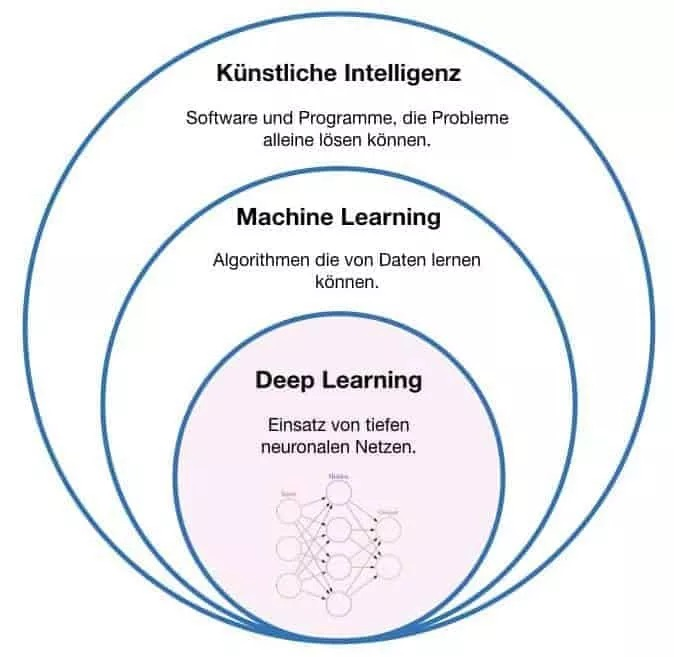
\includegraphics[width=0.5\textwidth]{ki-aufbau.jpg}
    \caption{Aufbau der KI}
    \label{fig:ki-aufbau}
\end{figure}

\section{Maschinelles Lernen}
Die KI verwendet \textbf{Maschinelles Lernen}. Damit kann der Computer automatisiert lernen. Er kann sich dabei ständig verbessern und seine Fähigkeiten verfeinern.
Für diese Methode werden Algorithmen verwendet, die Beziehungen zwischen Variablen (d. h. Muster) entdecken und dann aus diesen Lektionen lernen. Je mehr Daten sie erhalten, desto effizienter wird die KI.

\subsection{Deep Learning}
Beim \textbf{Deep Learning}-Verfahren werden \textbf{neuronale Netze} verwendet.
Neuronale Netze ahmen die Funktionsweise des menschliche Gehirns durch Algorithmen nach. Sie können aus Datenquellen Informationen und Muster erkennen und diese auf unbekannte Daten anwenden.
Das \textit{Deep Learning} wird dazu verwendet, um Bilder zu erkennen, Texte zu verstehen und Entscheidungen genauer zu tätigen.

\section{Training in drei Schritten}
Das Training einer KI ist in folgende drei Schritte aufgeteilt.

\subsection{Training}
Im ersten Schritt wird der Computer mit Daten gefüttert. Algorithmen können die Daten analysieren um bessere Vorhersagen zu treffen und die Genauigkeit von denen zu bewerten. Dafür wird das maschinelle Lernen angewandt.
Für das KI-Training gibt es zwei Methoden: überwachtes und unüberwachtes Lernen.
\\
\textbf{Überwachtes Lernen} Die Eingebedaten werden von einer Person geeignet gekennzeichnet, damit dem Computer keine Verwechslungen unterlaufen.
\\
\textbf{Unüberwachtes Lernen:} Beim unüberwachten Lernen gibt es wiederum drei Arten:  Clustering, Association Rule Mining (Assoziationsregel-Mining) und Ausreissererkennung. Beim \textit{Clustering} werden nicht gelabelte Daten nach bestimmten Kriterien zusammengefasst, indem die KI Ähnlichkeiten und Unterschiede mit den bereits gelabelten Daten sucht.
Durch das \textit{Association Rule Mining} werden die Daten etwas anderes betrachtet, mit der Absicht, Beziehungen zwischen Datenpunkten und verschiedenen Elementgruppen zu finden.
Die \textit{Ausreissererkennunng} wird verwendet, um Anomalien in Datensätzen zu finden, die außerhalb bestimmter Grenzen liegen.

\subsection{Validierung}
Im Valiedierungstest wird die Genauigkeit der KI mit den Testdaten verglichen. Damit kann man feststellen, ob die KI weiteres Training braucht oder bereit ist.

\subsection{Test}
Der KI werden unstrukturierte Datensätze (d.h. ohne Tags oder Ziele) gegeben. Nachdem sie darauf trainiert ist, wird sie auf die Probe gestellt. Je genauer die Entscheidungen sind, desto besser sind Sie vorbereitet, wenn sie in Betrieb geht.

\section{Quellen} \citep{KI-Training}, \citep{neuronale-netze}